\documentclass[10pt, conference]{IEEEtran}
\IEEEoverridecommandlockouts
% The preceding line is only needed to identify funding in the first footnote. If that is unneeded, please comment it out.
\usepackage{cite}
\usepackage{amsmath,amssymb,amsfonts}
\usepackage{algorithmic}
\usepackage{graphicx}
\graphicspath{ {images/} }
\usepackage{textcomp}
\usepackage{listings}
\usepackage{color}
\usepackage{hyperref}

\definecolor{dkgreen}{rgb}{0,0.6,0}
\definecolor{gray}{rgb}{0.5,0.5,0.5}
\definecolor{mauve}{rgb}{0.58,0,0.82}

\lstset{frame=tb,
  language=Java,
  aboveskip=3mm,
  belowskip=3mm,
  showstringspaces=false,
  columns=flexible,
  basicstyle={\small\ttfamily},
  numbers=none,
  numberstyle=\tiny\color{gray},
  keywordstyle=\color{blue},
  commentstyle=\color{dkgreen},
  stringstyle=\color{mauve},
  breaklines=true,
  breakatwhitespace=true,
  tabsize=3
}
\usepackage{xcolor}
\def\BibTeX{{\rm B\kern-.05em{\sc i\kern-.025em b}\kern-.08em
    T\kern-.1667em\lower.7ex\hbox{E}\kern-.125emX}}
\begin{document}

\title{Beginner's Guide to Serverless: AWS Lamda vs. Google Cloud Functions\\}

\author{
\IEEEauthorblockN{1\textsuperscript{st} Falkner, Alexandra}
\IEEEauthorblockA{\textit{Dept of EECS} \\
\textit{Vanderbilt University}\\
New York, USA \\
alexandra.falkner@vanderbilt.edu}
\and
\IEEEauthorblockN{2\textsuperscript{nd} Wolfe, Parish}
\IEEEauthorblockA{\textit{Dept of EECS} \\
\textit{Vanderbilt University}\\
NC, USA \\
parish.wolfe@vanderbilt.edu}

}

\maketitle

\begin{abstract}
Architecture composed of serverless functions is becoming more and more popular as more businesses embrace the cloud. With this expansion in mind, this paper serves as a beginners guide to serverless computing. The purpose of this paper is to obtain an understanding of what serverless computing, specifically serverless functions, why someone would want to use it, and a comparison of two of the most popular serverless computing platforms - AWS Lamda, and Google Cloud Functions. 

\end{abstract}

\begin{IEEEkeywords}
serverless computing, serverless functions
\end{IEEEkeywords}

\section{Serverless Overview}
\subsection{What is Serverless Computing?}
Serverless computing is a cloud-native development model that allows for the deployment of applications on cloud infrastructure without the need to maintain servers. With serverless, a chosen cloud provider is responsible for handling the provisioning, maintenence, and scaling of the server infrastructure, while users are simply responsible for deploying code on the cloud environment. 

Serverless computing is comprised of two groups. Firstly, Backend as service (BaaS), and secondly, Function as a service (Faas) \cite{b1}. BaaS offers users services that automate the backend of development. While, FaaS gives users the ability to execute code in response to events in cloud without having to maintain the cloud infastructure. FaaS is the type of serverless computing we will be focusing on in this paper. Often the terms FaaS and serverless are used synonymously. 

As the name implies, the intended use for one serverless function is equivalent to one function of an application. Serverless functions are event driven, and are instantiated when the event occurs. Most commonly, serverless functions are short-lived, stateless and have a single-purpose \cite{b2}. When some event occurs on the cloud platform, the function associated with that event is triggered and is executed. When a serverless function is triggered information associated with the event is passed into the function as a parameter. 

A common pairing is for serverless functions to be triggered with a hypertext transport protocol (HTTP) request. Frequently, the inputs to a serverless function are applied with request headers, request body payload, or even request parameters. Support varies between providers. The most popular closed source providers are Amazon Web Services Lambda and Google Cloud Platform Cloud Functions, which we will discuss in detail here. Other notable providers are Microsoft Azure Functions, Oracle Functions, IBM Cloud Functions, CloudFlare Workers, and the open source do-it-yourself serverless platform, KNative.


\subsection{Benefits of Serverless Computing}
There are a multitude of reasons many companies are transitioning to serverless computing. In this section we will examine the main benefits that serverless functions provide. 

To begin, a benefit of utilizing a serverless platform is improved scalability. Traditional cloud servers take a considerable amount of time to bring up and down. Serverless code launches in seconds, not minutes like cloud virtualized servers. This is in a large part due to the fact that cloud providers for serverless platforms use containers, a technology that allows for fast start-up times. Serverless functions are seemingly infinitely horizontally scalable with a negligible amount of time involved to provision a new instance. Consequently, a user is able to scale automatically up or down as needed, with little time and effort. 

Another particularly argument in favor of serverless computing is the cost. A user will only pay for the resources used, and with serverless's easily flexible scalability this means a user is only paying for the resources they need. The cost can be a stark contrast compared to more traditional cloud offerings like Amazon EC2. Serverless is very inexpensive, because you are not paying to run an operating system, only for the code execution. In fringe cases, this can be problematic if you require binaries compiled in an obscure language. Serverless offerings across the board cover a majority of users' needs with support for most every popular programming language, to include java, python, javascript and more. 

Perhaps the most obvious benefit of serverless is that no server management is required from the user. The servers used in serverless computing are all managed by the cloud providers. As a result, this can further save institutions money that would previously be spent on DevOps, but also uncomplicates the process so that developers can spend their time focusing on other company ventures. 

I mentioned above the time saved in serverless during start-up with containers, but to expand on this there is an additional time saver as users are able to quickly upload code without the need for background configuration. This makes it possible to quickly update, patch, fix, or add new features. 

Once deployed, serverless apps respond to demand and automatically scale up and down as needed. Serverless offerings from public cloud providers are usually metered on-demand through an event-driven execution model. As a result, when a serverless function is sitting idle, it doesn’t cost anything.

More abstractly, the nature of serverless functions requires a user to breakdown their work into sub-pieces. This decomposition can be great to gain a better understanding of a system and make it more observable. 

Lastly, a serverless platforms have error isolation. Serverless functions are event-based with each function independent of one another, and so if there is a failure within one sub-piece, only that piece is affected. This can make debugging easier as finding the route of the problem is a much less vexing process. 

\subsection{Drawbacks of Serverless Computing}

While there are many reasons to transition to serverless computing, there are important drawbacks to consider before making such a choice. 

Firstly, debugging can be a more difficult process. While locating the function that has failed is seamless, replicating a serverless environment can be near impossible. As a result, debugging becomes a complex process when a developer has no visibility of the backend processes and cloud environment.

Secondly, and possibly the most poignant issue for companies is that serverless architecture open up a system to whole new security concerns. Depending on a companies security measures, a provider might not be able to match their security needs on the backend. With serverless, most security concerns are handed off and managed by the provider. With some institutions this can be beneficial as likely the security provided at Amazon and Google is far better than any security system they could build. However, this system does create a larger attack plain with more entry points into the server. Serverless computing creates one big target for attackers to focus on, and if they succeed the users are largely powerless in fixing the issue. Additionally, due to the nature of serverless a given company is not designated a certain set of servers. Often there will be multiple users functions running on one server. This sharing of machinery is known as multitenancy, and brings with it a multitude of issues. For one, if not configured correctly it can effect application performance, and more concerningly, result in data exposures. 

Additionally, there are scenarios where serverless is not cost effective. This can happen with long-running processes. Serverless providers charge a user by the time they use their service, and so if a company requires many long-running processes this can become costly, fast. In cases such as this it is often more economic to use a traditional server infrastructure. 

Lastly, while serverless is known for being fast, there are areas that can be time costly. If a function has not be used in a while, when triggered there will be what is referred to as a cold start. This requires the server to boot up the code, and is comparably slower than requests without a cold start. 

\section{Serverless Comparison}

This section of the paper will offer important insights into and comparisons with AWS Lamda and Google Cloud Functions. We chose to compare these two platforms as they are within the 3 most popular closed source options for serverless computing, especially for beginners \cite{b4}. 

\subsection{Pricing}

AWS Lambda is included in AWS's Compute Savings Plans, a more flexible pricing model that offers lower prices for a longer commitment to a consistent amount of usage[cite]. Instead of agreeing to use the platform at an hourly rate, the user will commit to a contract anywhere from one to three years long. In doing so they can create great saving for themselves. 

With the On-Demand rate an AWS user is given 1 million requests per month free. Every 1 million requests after has an additional cost of \$0.20, or you can pay \$0.0000002 for each additional individual request. An AWS Lambda user is given 400,000 GB-seconds of compute time per month free, with each GB-second used after being \$0.00001667. 

Google Cloud Functions provide a free tier similar to AWS Lambda and then two tiers afterwards that depend on the region you are running your function in. These two tiers affect the compute time pricing. Each user is given 2 million free requests per month, with each a million requests afterwards being \$0.40, or each individual additional request being \$0.0000004. Similar to AWS Lambda, Google Cloud Functions offers 400,000 GB-seconds per month free. In Tier 1 each GB-second costs \$0.0000025, and in Tier 2 \$0.0000035. 

It should be noted that for both AWS Lambda and Google Cloud Functions, computing time prices are variable based on the amount of memory and CPU provisioned for the function. 

\begin{figure}[htbp]
\centerline{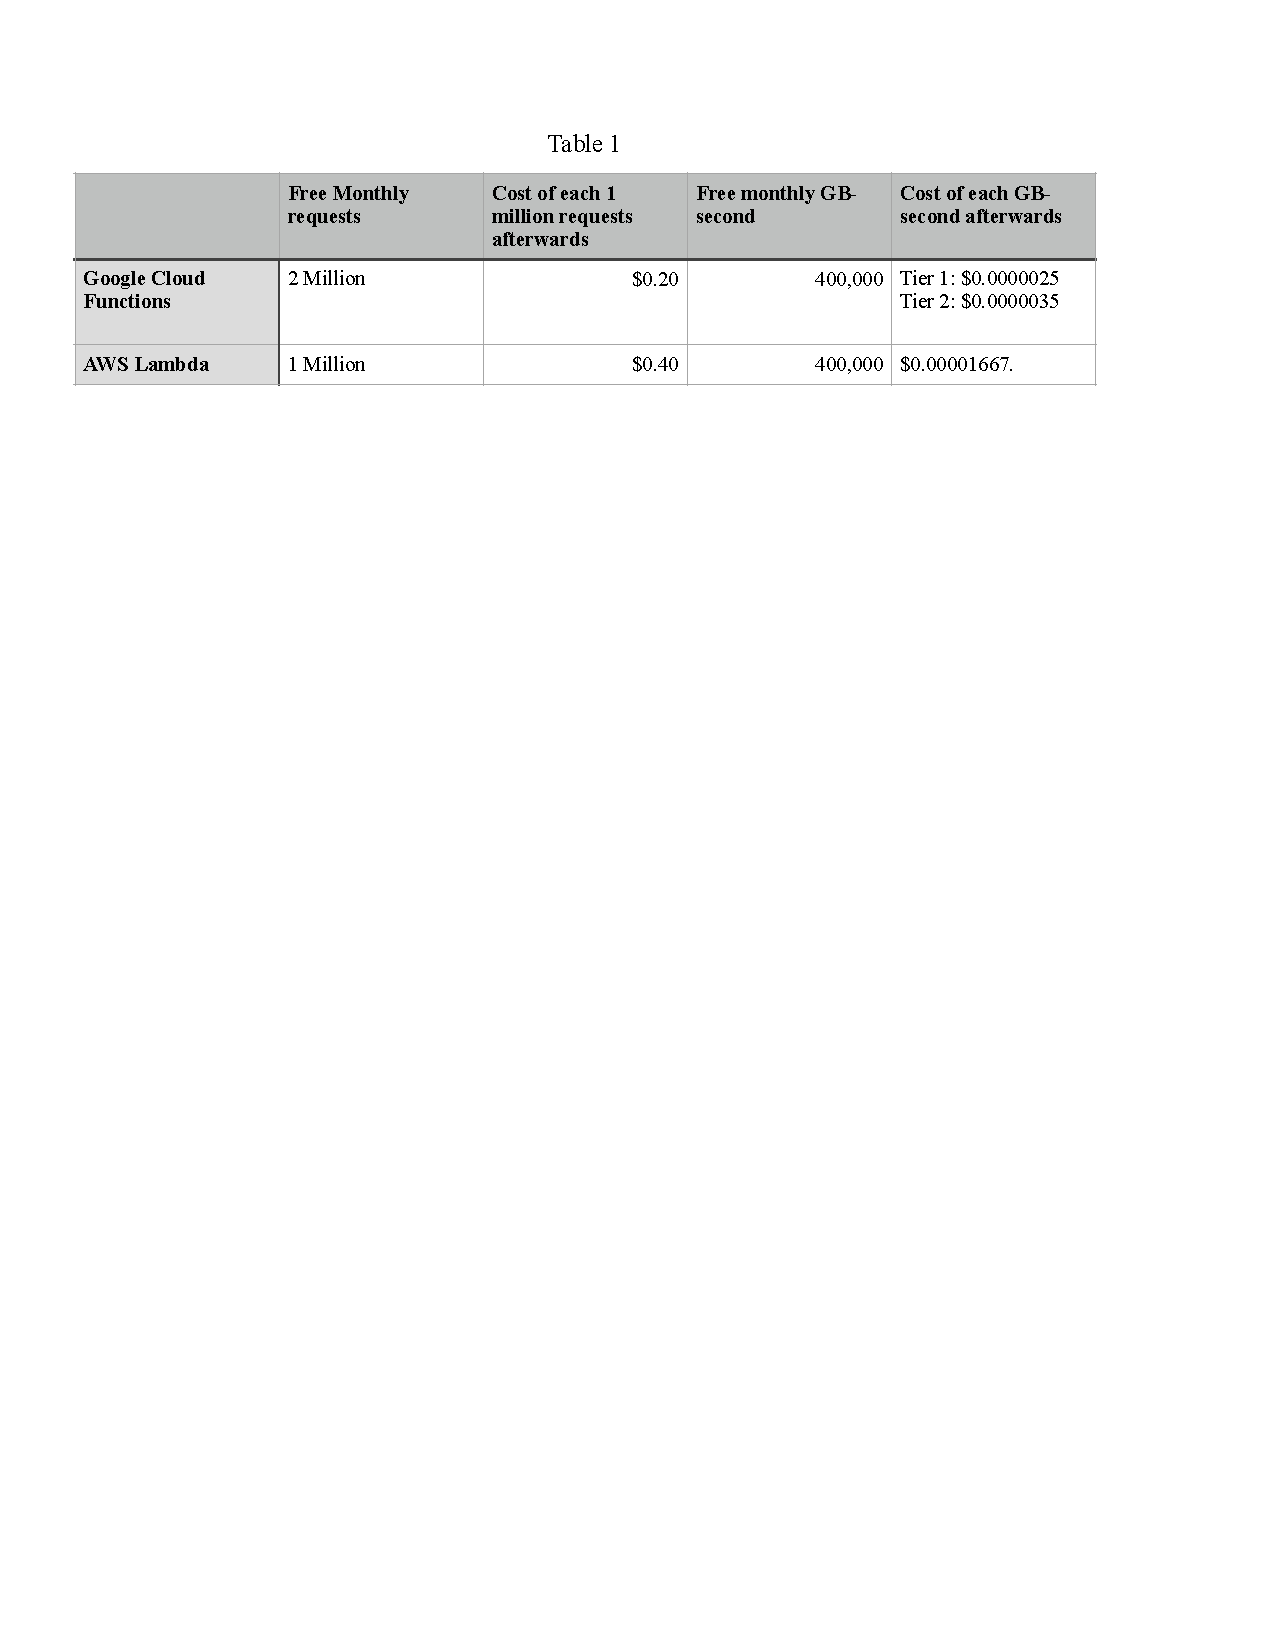
\includegraphics[width=9cm]{table1.PDF}}
\caption{Price Comparison AWS Lambda vs. Google Cloud Functions.}
\label{fig}
\end{figure}

\subsection{Configuration and Performance}

AWS Lamda, and Google Cloud Functions both provide slight variations when it comes to configuration and performance. 

To begin, Google Cloud Functions has a longer cold start time. A cold start occurs when a function is first run or has been idle. In tests performed by Cloud Developer and researcher Mikhail Shilkov, AWS Lamda's cold starts averaged to be less than 0.5 seconds, with Google Cloud Functions averaging 0.5 - 2 seconds. The timing for cold starts varies among execution environments, but in our tests discussed later in this paper we found our data to be the same as that given above. 

Google Cloud Functions and AWS Lambda offer different memory configurations. Google Cloud Functions offers 128MB - 8192MB going up in multiples of 128 MB. However, AWS Lambda offers a more impressive range of 128MB - 10240MB. 

In addition Google Cloud Functions time out after a maximum 9 minutes of execution [b5], while AWS Lambda functions time out after 15 minutes. This longer limit on execution time, and more robust memory offering mean that AWS Lambda is better equipped to handle larger loads. 

\section{Google Cloud Functions}

Google Cloud Functions is a serverless execution environment for building and connecting cloud services. It was launched in April 2016 and has since become one of the most popular serverless execution environments out there. 

\subsection{How does it work?}

The user will choose the execution environment, either from those provided by Google Cloud Functions, or by making a custom image. Then, after writing their function they can deploy it easily using Google Cloud Function's SDK. 

\subsection{Execution Runtime}

Google Cloud Functions support numerous language runtimes. The runtimes currently available are Node.js, Python, Go, Java, .NET Core 3.1, Ruby and PHP. Additionally a user can create and use their own custom runtime using Docker images. 

\subsection{What events can trigger a function?}

To execute your serverless function, there must be an event that triggers it in your cloud environment. These events can range from changes to data in a database to a new virtual machine being created. Google Cloud Functions supports events from the following providers: HTTP, Cloud Storage, Cloud Pub/Sub, Cloud Firestore, Firebase, and Cloud Logging.

An HTTP(s) request will trigger a HTTP function, and other events will trigger what are called event-driven functions. There are two types of event-driven functions, background functions, and CloudEvent functions. 

\subsection{HTTP Functions}

HTTP functions are used when the events associated with a function is an HTTP(s) request. A user is able to specify whether they would like HTTPS events only to trigger a function. If a user chooses to do so, then any person using the HTTP protocol instead of the HTTPS protocol will be redirected. 

\subsection{Background Functions}

A background function is a type of event-driven function. Google Cloud's background functions support Node.js, Go, Python and Java. These type of functions are utilized when a user wants to execute their function indirectly to the event [cite]. This means they will be executed as part of event triggers that occur in supported Google Cloud Platform Event Providers \cite{b7}. An example of such an event could be a message on a Pub/Sub topic. Cloud Pub/Sub is a messaging middleware that is part of the Google Cloud Platform. 

As mentioned prior the arguments in Google's serverless functions pass information about the event associated with the function. In a python environment, the function parameters for a background function will be \verb|{(data, context)}| as shown in \ref{fig:param}. Data is a dictionary that contains the data for the event. The format of this dictionary will depend on the event. The parameters are very similar for all other environments. 

\begin{figure}[htbp]
\centerline{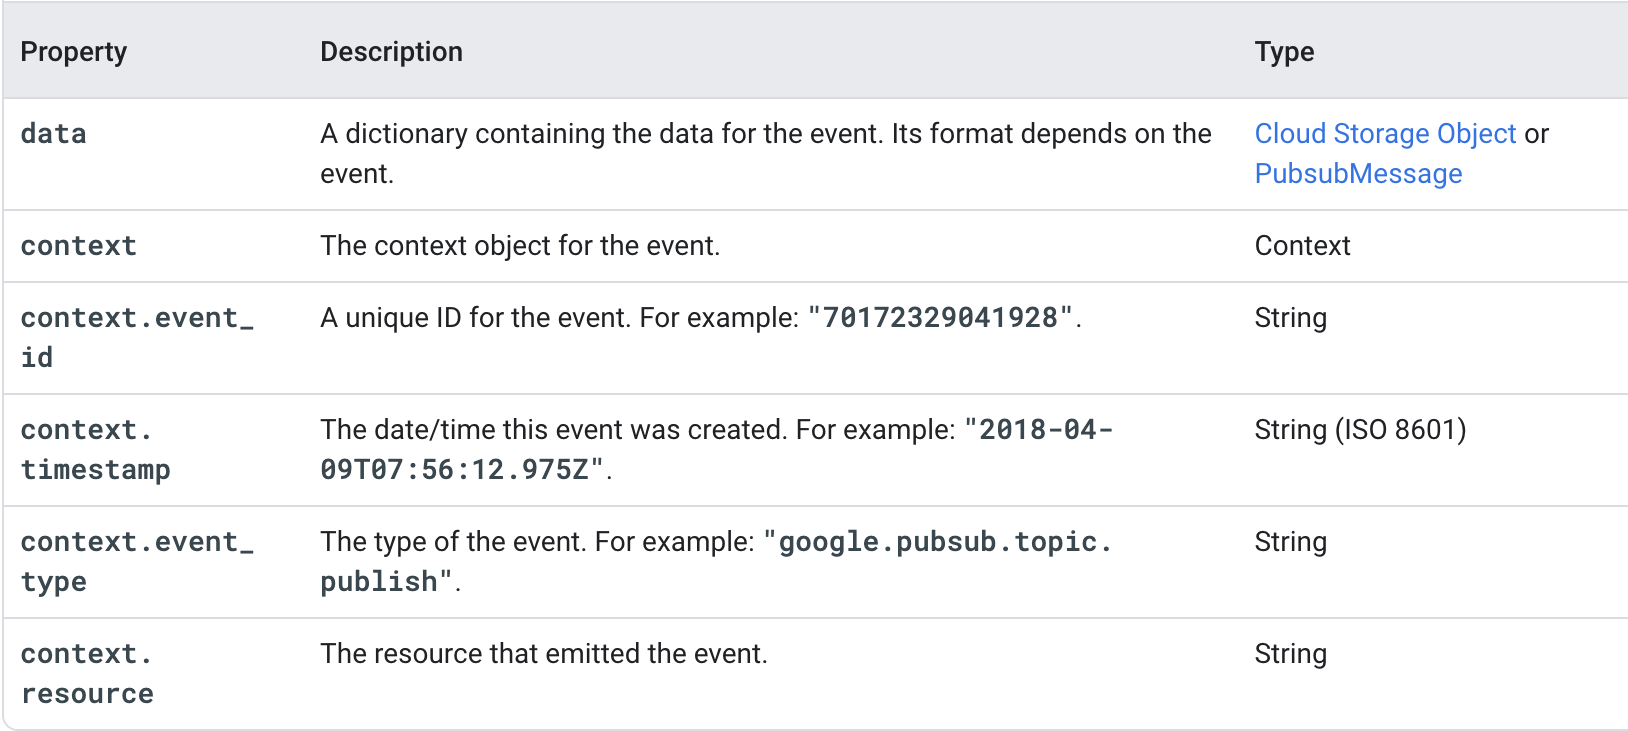
\includegraphics[width=9cm]{background_parameters.PNG}}
\caption{Parameters for Background Function in Python Environment \cite{b6}.}
\label{fig:param}
\end{figure}

\subsection{CloudEvent Functions}

A Cloud Event function is the second type of event-driven function. Like background functions, CloudEvent functions are triggered indirectly by an event. However, CloudEvents functions use an industry-standard event format known as CloudEvents. CloudEvents is a specification for describing event data so that they are comparable in a common way. CloudEvent functions support PHP, C\#, and Ruby. CloudEvent functions have the parameter, a cloudEvent object as seen in \ref{fig:param2}. This holds all the metadata associated with the event.

\begin{figure}[htbp]
\centerline{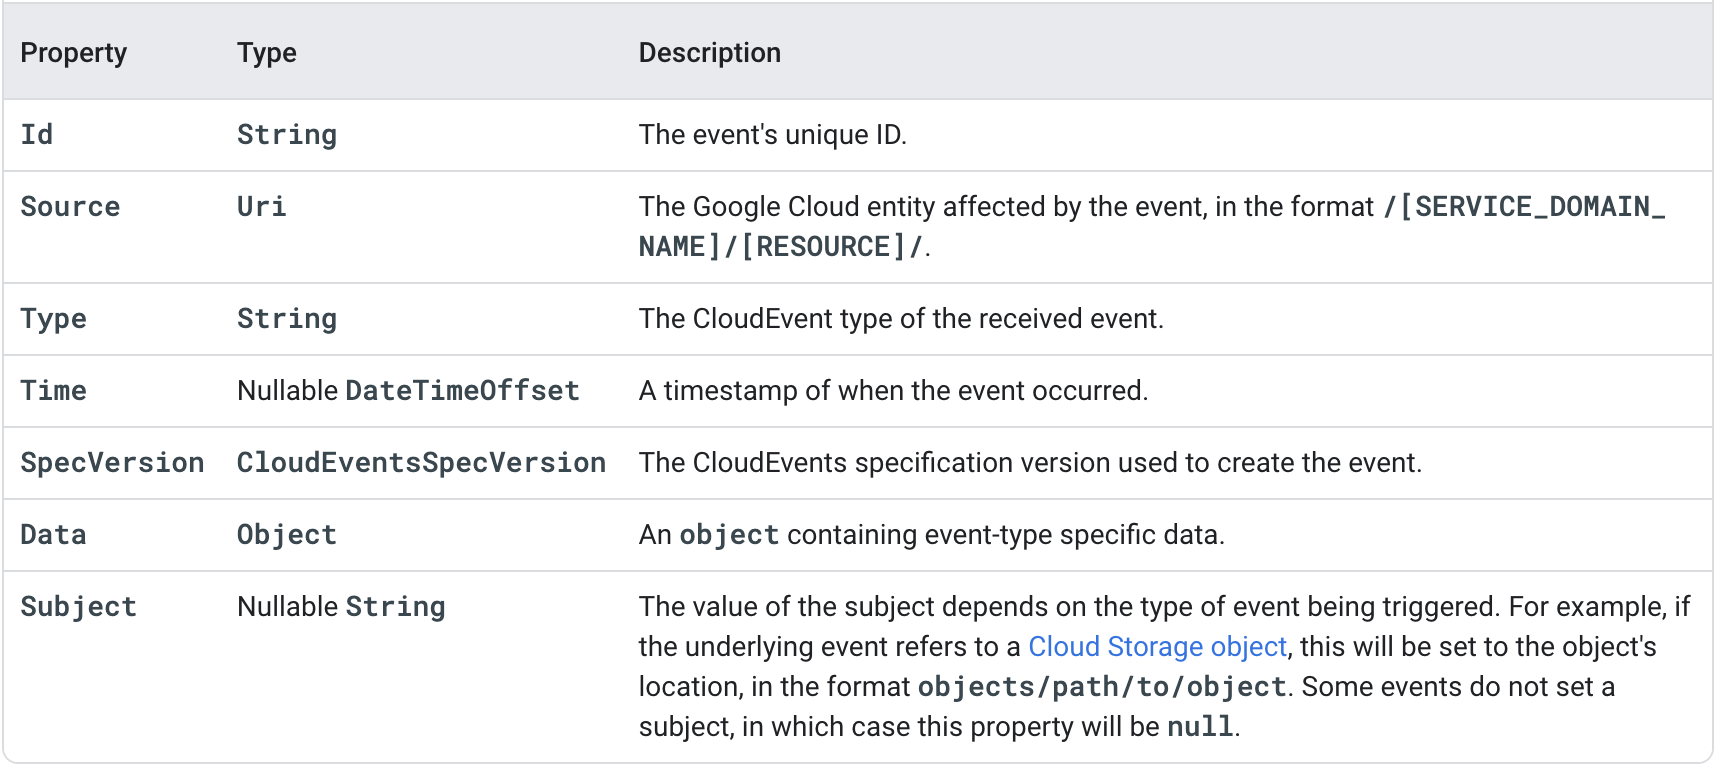
\includegraphics[width=9cm]{cloudEvent.PNG}}
\caption{The properties of a cloudEvent object.}
\label{fig:param2}
\end{figure}

\subsection{Cloud Function Images }

When a function is deployed, the source code is stored in a Cloud Storage bucket. Cloud Built then automatically builds this into a container image that is put into the Container Registry or the Artifact Registry if specified at deployment. Hence, Cloud Functions can access this image and run the container to execute the function. 

Due to images being automatically created, Google Cloud Functions create an easier experience for its users. 

\section{ AWS Lambda}
AWS Lambda was released in 2014, and has since been a major player in the world of serverless computing. 
\subsection{How does it work?}

Lambda offers several options to create a function. Those options are to write code from scratch, use a blueprint, container image, or launch a prebuilt lambda function from the AWS serverless application repository.

\subsection{Execution Runtime}

The most common use case is to write a lambda function from scratch. The first step is to select a runtime. This is analogous to choosing what language your code is written in. Options include python, nodejs, java, C\#, Go, and Ruby. There is an option to bring in your own custom runtime with the stipulation that it must run on amazon linux.

\subsection{Container Image}
Another great option offered by Lambda is the ability to create a function based on a container image. This gives a user the ability of nearly infinite customization. With this option one could even write serverless in Fortran if the need ever made sense. This allows for any container to be executed as a lambda function. 

\subsection{Blueprints and Serverless App Repository}
These are additional options available when creating a function. Blueprints are prewritten code for common use cases. The serverless app repository is a collection of ready to deploy applications that meet specific use cases. There are many great serverless examples, and the option to create a private application not open to the public. 

\subsection{What events can trigger a function?}
The most common type of trigger is an http request, which will be discussed in greater detail in the following section. Many types of events can trigger an AWS lambda function. Modification of data in S3 buckets or in dynamo db can be events as well as Cognito, ELB, connect, Lex, Alexa, Cloudfront, Kinesis, and Simple Storage. 

\subsection{HTTP Functions}
Unlike many other providers, lambda functions are not configured to accept http requests as an event by default. Amazon API Gateway must be paired with Lambda to start a lambda function with an http request. This is an additional service, with an additional cost, but allows for great flexibility.

\section{ Experiments}
In this section of our paper we will lay out and analyze experiments performed on AWS Lambda and Google Cloud Functions. This will give insight into the capacity and user experience of both platforms. For our experiments we used HTTP functions, as they had the most easily comparable architecture and design. 

\subsection{Design I}
The first experiment we created an HTTP function that was triggered by HTTP requests. Google Cloud Functions you can download a Google Cloud SDK, \verb|gcloud| and use the following command to deploy the function: 

\begin{lstlisting}
gcloud functions deploy FUNCTION_NAME --runtime RUNTIME_ENVIRONMENT --trigger-http
\end{lstlisting}

Then, use a cURL command to invoke the function. Below is an example of a POST request. 
\begin{lstlisting}
curl -X POST "https://YOUR_REGION-YOUR_PROJECT_ID
.cloudfunctions.net/FUNCTION_NAME" 
-H "Content-Type:application/json" 
--data '{"name":"Cloud Computing"}'
\end{lstlisting}


\subsection{Results I}

\begin{figure}[!htbp]
\centerline{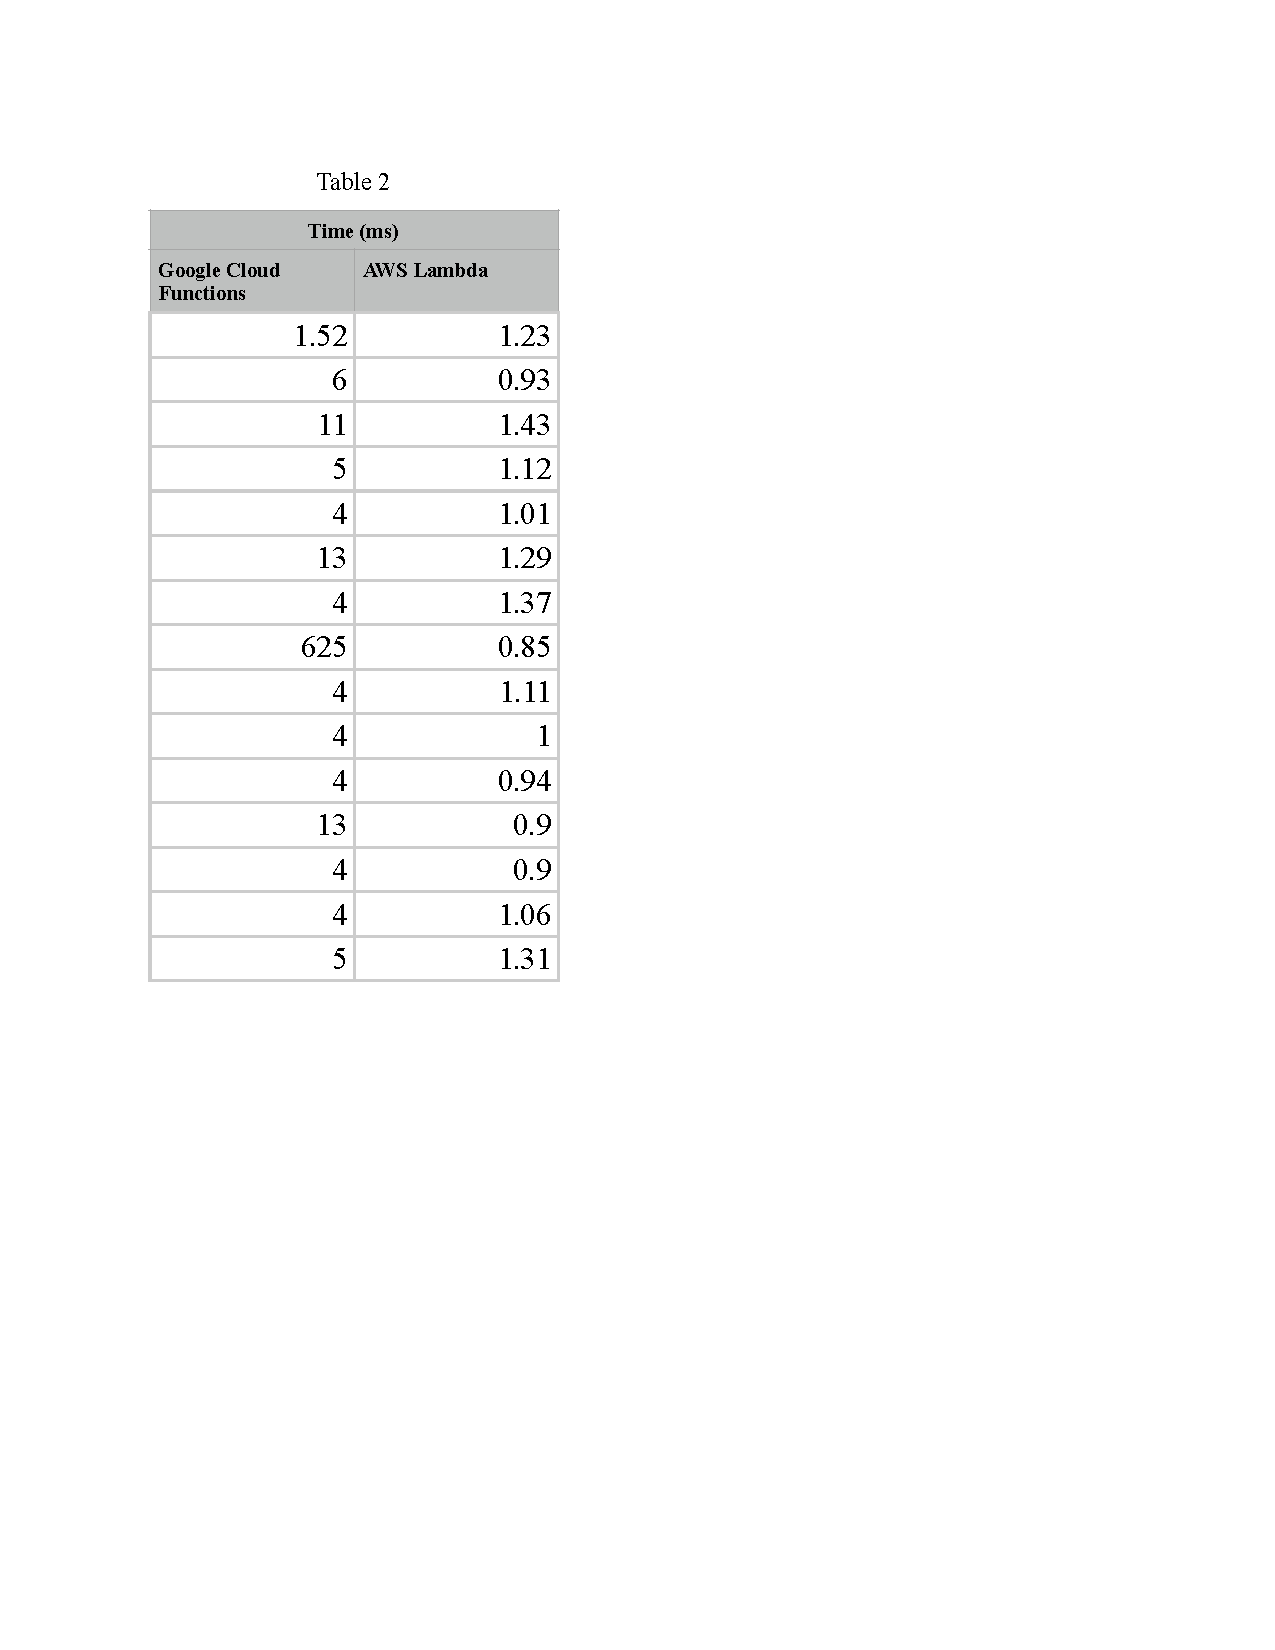
\includegraphics[width=6.5cm]{table2.PDF}}
\caption{Time for 15 HTTP functions in Google Cloud Functions and AWS Lambda}
\label{fig:tabletwo}
\end{figure}

The table shows the time (ms) it took for 15 requests to complete the functions. We replicated the test 10 times, and what you see is the average of those tests for each result. 

As you can see in \autoref{fig:tabletwo} Google Cloud Functions has a much higher cold start time. When the functions are initially ran, either for the first time, or after an idle period, the function takes considerably longer. Additionally, even disregarding the initial start-up time, AWS Lambda ran all other functions considerably faster as well. 

\subsection{Design II}
In our second experiment we timed response times for Google Cloud Functions and AWS Lambda for an HTTP Function that processed data. 

\subsection{Results II}
This experiment was repeated 10 times, and the results you see are the average of each 15 requests. 

\begin{figure}[!htbp]
\centerline{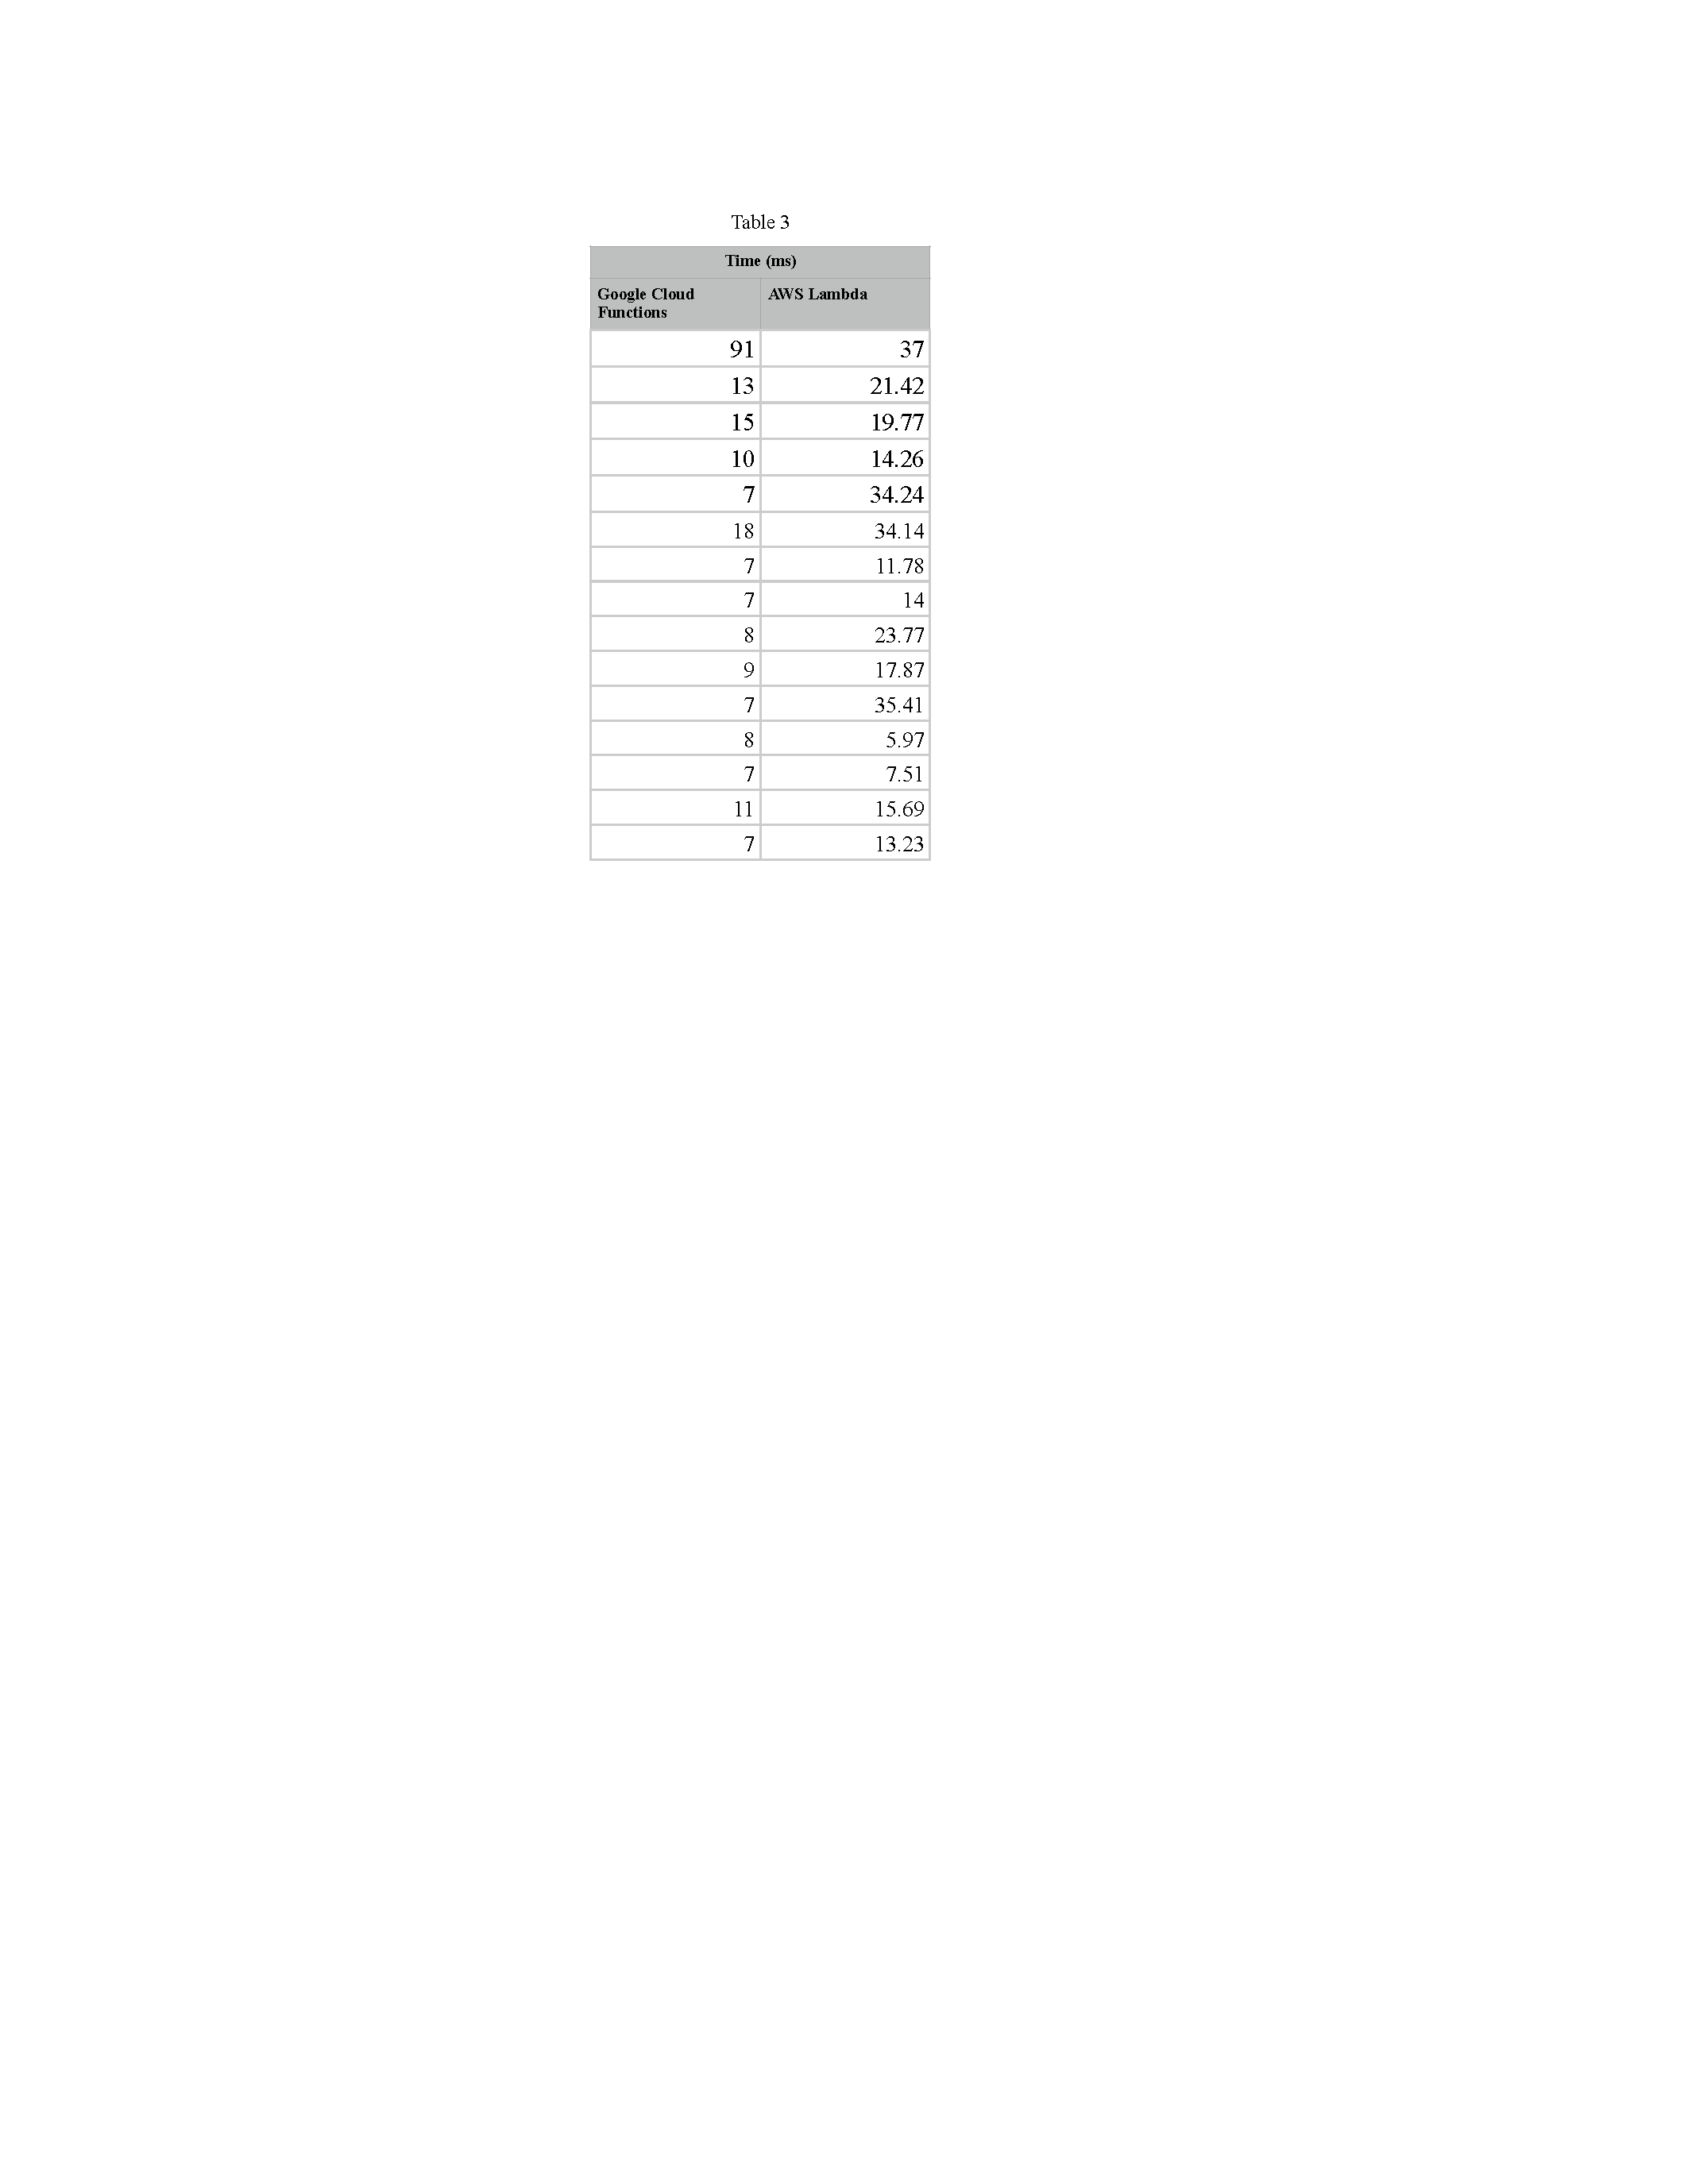
\includegraphics[width=7cm]{table3.PDF}}
\caption{Time for 15 functions in Google Cloud Functions and AWS Lambda}
\label{fig:table3}
\end{figure}

As seen in \autoref{fig:table3} with this experiment, we saw an entirely different result, whereby, Google Cloud Functions was noticeably faster at processing data. 

\subsection{Experiment Conclusion}

\begin{figure}[htbp]
\centerline{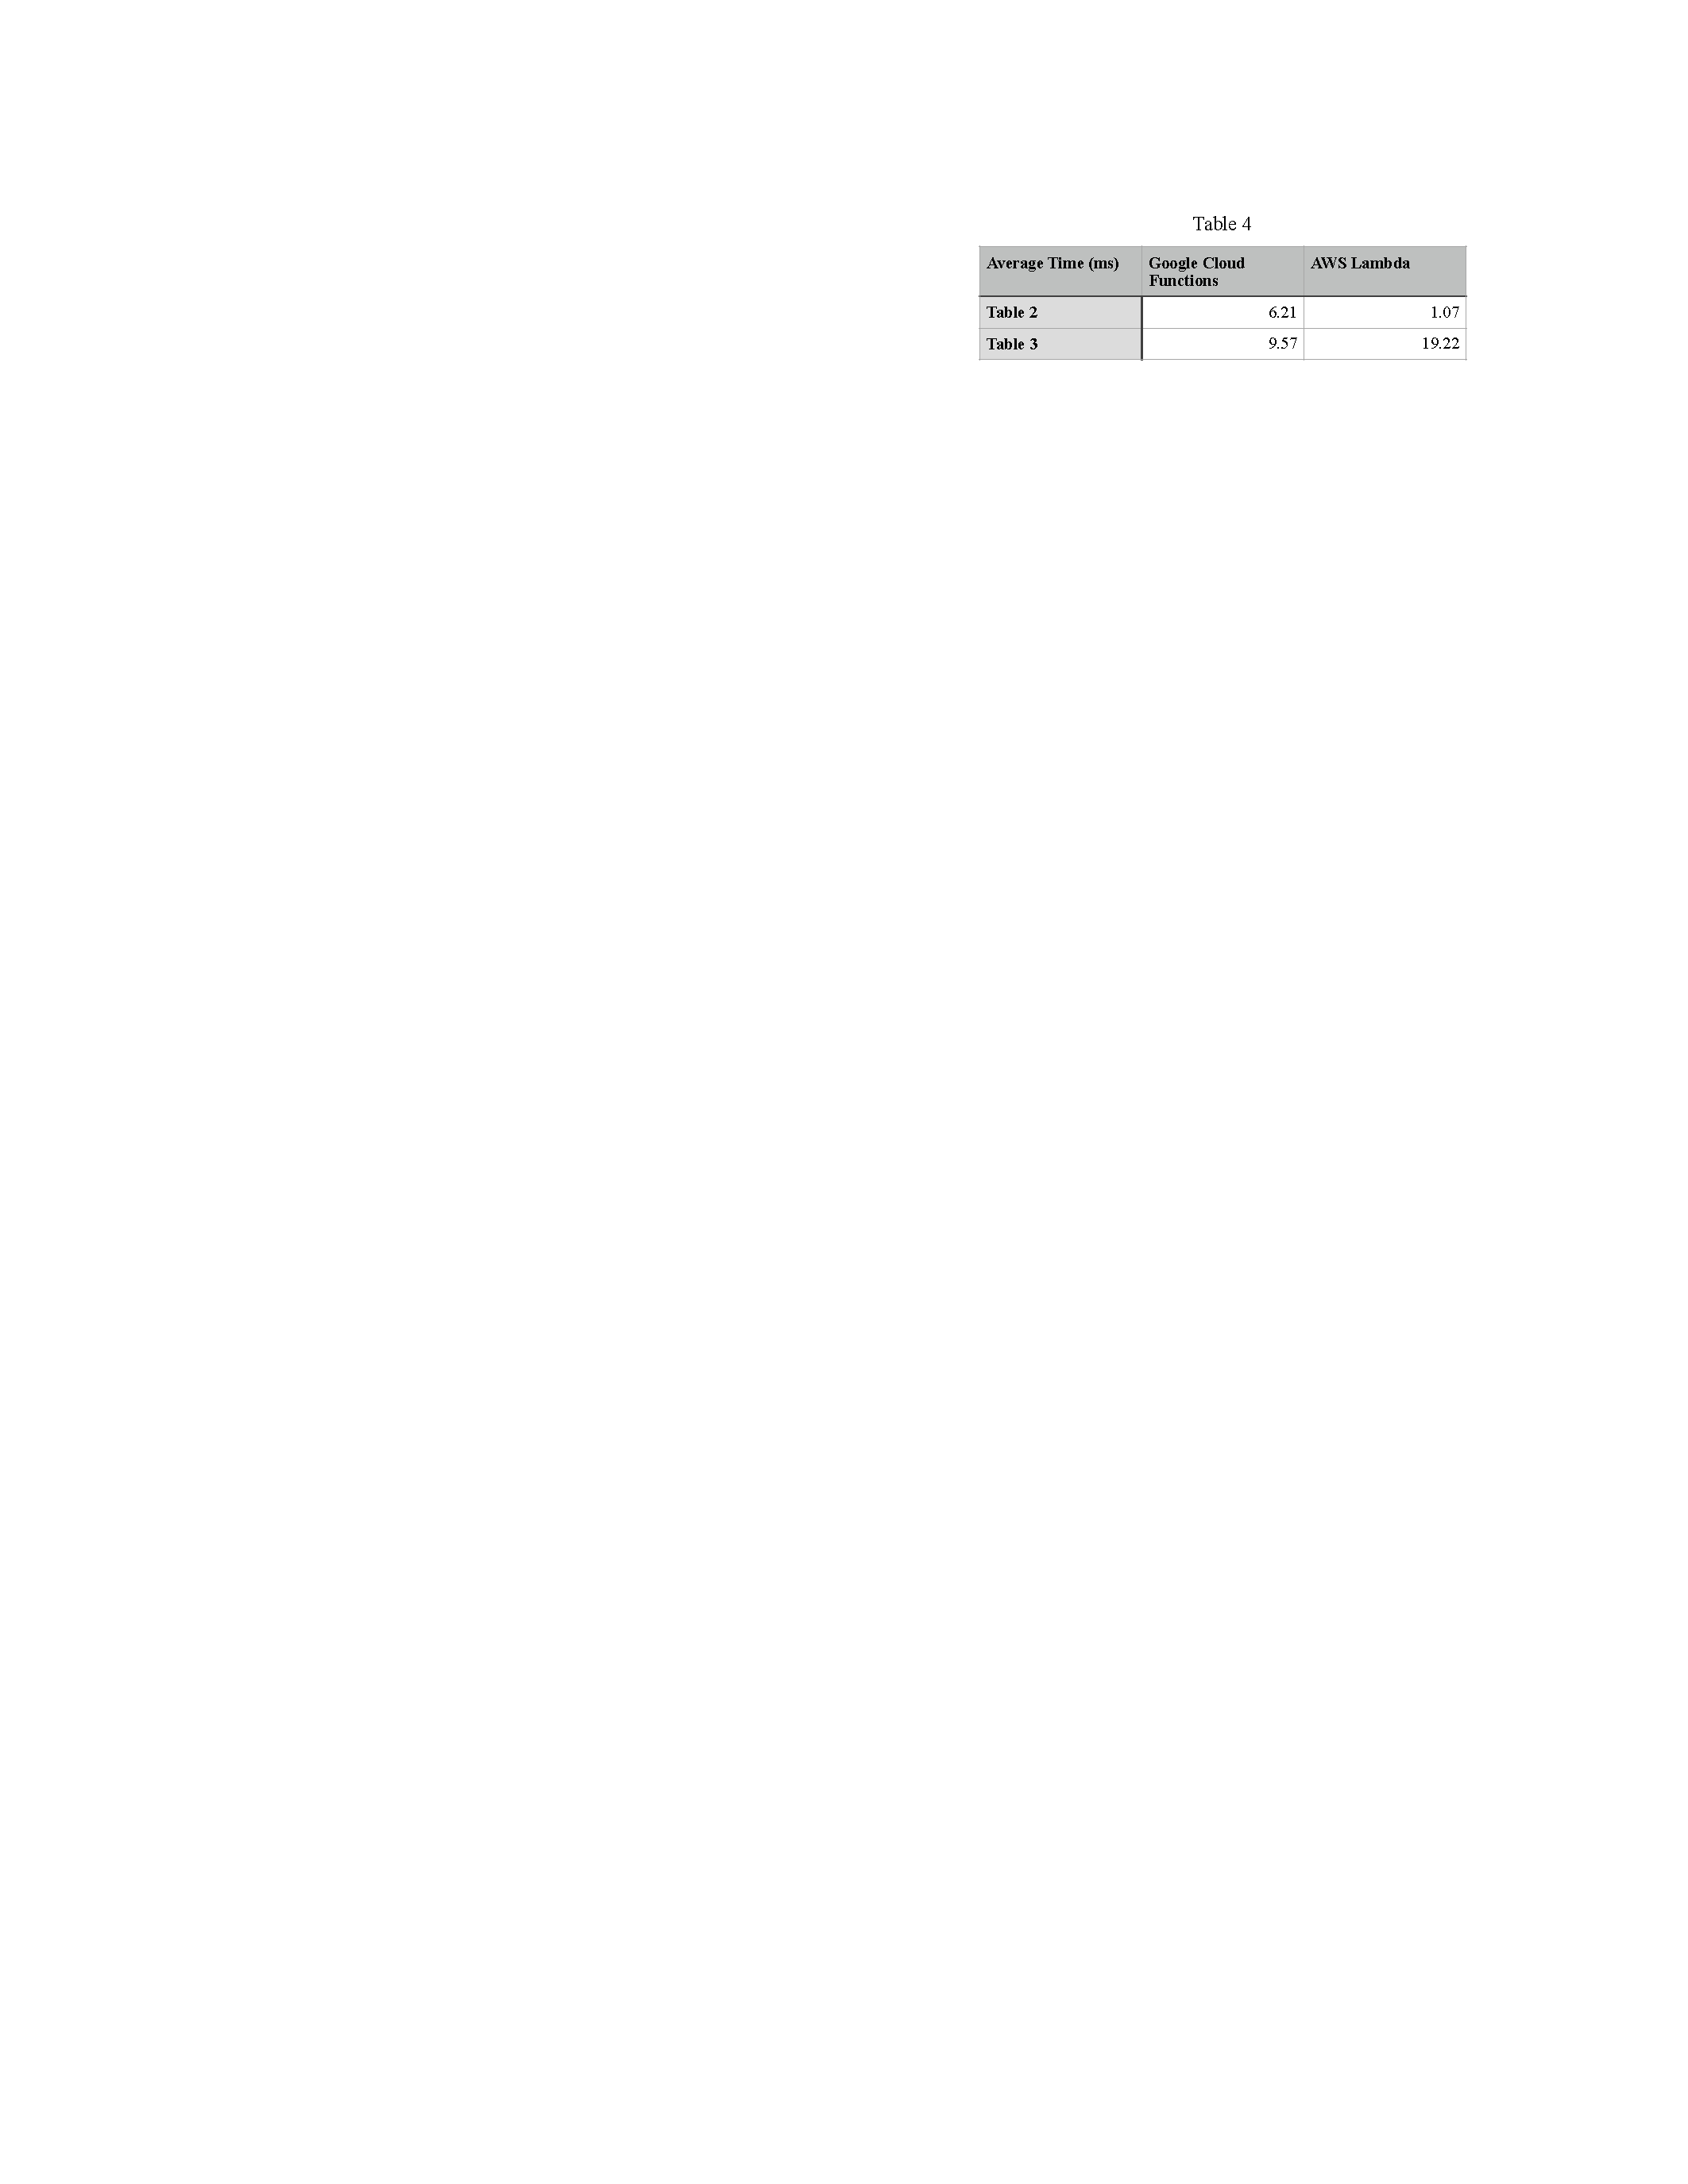
\includegraphics[width=9cm]{table4.PDF}}
\caption{Average Time for AWS Lambda and Google Cloud Functions from Table 2 and Table 3.}
\label{fig:table4}
\end{figure}


\subsection{User Experience}

Taking a step back from the results of our experiments, in performing them we learned important notes on the user experience of each platform. 

Firstly, building images for function was an easier process with Google Cloud Functions. With Google Cloud Functions it is required to create a repository in the Google Cloud Repository, and then when you instantiate the function, the image is automatically created in that repository. 

However, for AWS Lambda a user must use Docker locally to built an image and push that image to an elastic container repository. Then in AWS Lambda, the user selects this repository. We found this process complicated, and encountered many errors a long the way. 

Secondly, adding packages in AWS Lamda is a more complex process than with Google Cloud Functions. With AWS Lamda, to use a package in your function a user is required to create a custom runtime environment. This can be complex, and take a considerable amount of time. However, using a package in a Google Cloud Function is a much more simple process. Each function when written has a requirements file. Using a package is as simple as adding it to the requirements file. 

Thirdly, HTTP functions in AWS Lambda require an API Gateway, which is billed separately, while Google Cloud Functions does not. 

Lastly, we found that signing up for an Google Cloud Function account was far easier too. This required a few clicks, and took around 2 minutes. Signing up for an AWS Lamda account required far more steps, and took more time. 

\section{Conclusion}

In conclusion both AWS Lamda and Google Cloud Functions are attractive platforms to use for serverless computing. However, Google Cloud Functions provides an easier interface and user experience for beginners. 

\begin{thebibliography}{00}
\bibitem{b1} Shafiel, Hossein ``Serverless Computing: A Survey of Opportunities,
Challenges, and Applications'', vol. 1, no. 1, pg 3, June 2021. 
\bibitem{b2} A Cloud Guru ``Orchestration” 2021. [Online]. Available: https://acloudguru.com/blog/engineering/serverless-showdown-aws-lambda-vs-azure-functions-vs-google-cloud-functions
\bibitem{b3} LoginRadius ``Top 4 Serverless Computing Platforms in 2021” 2021. [Online]. Available:  https://www.loginradius.com/blog/async/serverless-overview/
\bibitem{b4} Apache CouchDB ``ACID” 2021. [Online]. Available:  https://docs.couchdb.org/en/stable/intro/overview.html 
\bibitem{b5} Apache CouchDB ``ACID” 2021. [Online]. Available:  https://docs.couchdb.org/en/stable/intro/overview.html 
\bibitem{b6} Google Cloud ``Function Parameters” 2021. [Online]. Available:  https://cloud.google.com/functions/docs/writing/background\#functions \_background\_parameters-python
\bibitem{b7} Romin Irani’s Blog ``Google Cloud Functions Tutorial : Writing Background Functions” 2021. [Online]. Available:  https://rominirani.com/google-cloud-functions-tutorial-writing-background-functions-e651f27ddde5
\bibitem{b8} Apache CouchDB “ACID” 2021. [Online]. Available:  https://docs.couchdb.org/en/stable/intro/overview.html 
\bibitem{b9} Apache CouchDB “Introduction” 2021. [Online]. Available: https://docs.couchdb.org/en/main/ddocs/views/intro.html
\bibitem{b10} Apache CouchDB “What is a View?” 2021. [Online]. Available: https://docs.couchdb.org/en/main/ddocs/views/intro.html
\bibitem{b11} IBM “What is Map Reduce?” 2021. [Online]. Available: https://www.ibm.com/analytics/hadoop/mapreduce
\bibitem{b12} IBM “What is Map Reduce?” 2021. [Online]. Available: https://www.ibm.com/analytics/hadoop/mapreduce
\bibitem{b13} Apache CouchDB “CouchDB Replication” 2021. [Online]. Available: https://docs.couchdb.org/en/stable/replication/conflicts.html
\bibitem{b14} O'Reilly “Replication” 2021. [Online]. Available:  https://www.oreilly.com/library/view/couchdb-the-definitive/9780596158156/ch16.html 
\bibitem{b15} O'Reilly “Continuous Replication” 2021. [Online]. Available: https://www.oreilly.com/library/view/couchdb-the-definitive/9780596158156/ch16.html 
\bibitem{b16} Apache CouchDB “Distributed Updates and Replication” 2021. [Online]. Available: https://docs.couchdb.org/en/stable/intro/overview.html
\bibitem{b17} Apache CouchDB “Incremental Replication” 2021. [Online]. Available: https://docs.couchdb.org/en/stable/intro/consistency.html
\bibitem{b18} Apache CouchDB “Incremental Replication” 2021. [Online]. Available: https://docs.couchdb.org/en/stable/intro/consistency.html
\bibitem{b19} Apache CouchDB “Incremental Replication” 2021. [Online]. Available: https://docs.couchdb.org/en/stable/intro/consistency.html
\bibitem{b20} Apache CouchDB “Introduction” 2021. [Online]. Available: https://docs.couchdb.org/en/stable/cluster/sharding.html
\bibitem{b21} Apache CouchDB “Partitioned Databases” 2021. [Online]. Available: https://docs.couchdb.org/en/main/partitioned-dbs/index.html
\bibitem{b22} O'Reilly “Consistent Hashing” 2021. [Online]. Available: https://www.oreilly.com/library/view/couchdb-the-definitive/9780596158156/ch19.html 
\bibitem{b23} O'Reilly “Redundant Proxies” 2021. [Online]. Available: https://www.oreilly.com/library/view/couchdb-the-definitive/9780596158156/ch19.html 
\vspace{12pt}
\end{thebibliography}
\end{document}
